\section{AHTR Plank Optimization Results Discussion}
\label{sec:plank-discussion}
In this section, I conduct a deep-dive to understand the motivating factors for 
each individual objective, and how their combined effects result in the optimal 
reactor models found by the three-multi-objective optimization simulations. 

\subsection{Discussion: Minimize $PF_{total}$ Objective}
\label{sec:plank-discussion-pf}
\paragraph{Simulation p-1a}
For simulation p-1a, I conducted single-objective optimization 
simulations to minimize total fuel packing fraction ($PF_{total}$) by varying 
$PF_{total}$ and TRISO distribution. 
In simulation p-1a, \gls{ROLLO} found that an \gls{AHTR} plank model with a
$PF_{total}$ = 0.023 and oscillating TRISO distribution most-minimized 
$PF_{total}$ while meeting the $k_{eff} \geq 1.35$ constraint 
(Figure \ref{fig:slab-obj-1-pf}). 

I ran a simulation for constant $PF_{total}$ = 0.023 TRISO distribution and compared its 
fission reaction rate with the oscillating TRISO distribution 
to understand why the oscillating TRISO distribution enabled a lower $PF_{total}$. 
Figure \ref{fig:triso-0.023} shows the TRISO distributions for the two compared 
simulations: Figure \ref{fig:slab-obj-1-pf}'s most-minimized $PF_{total}$ 
and the constant $PF_{total}$ = 0.023. 
\begin{figure}[htbp!]
    \centering
    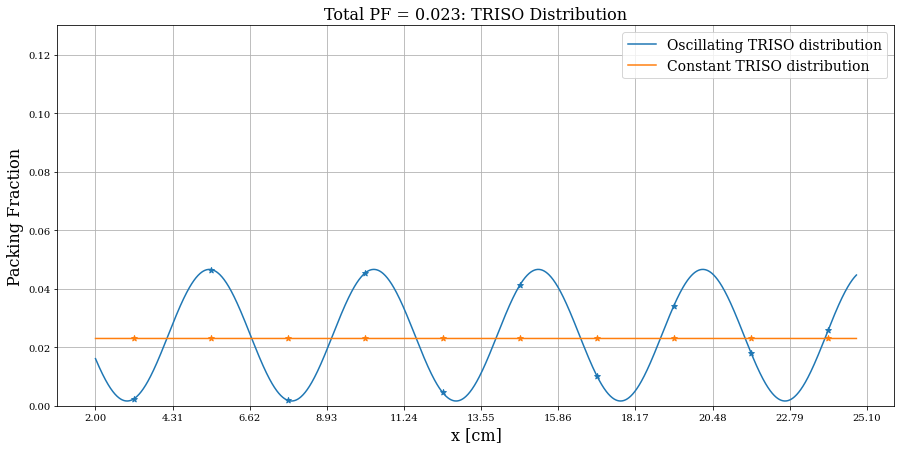
\includegraphics[width=0.9\linewidth]{triso-0.023.png} 
    \caption{Simulation p-1a's most-minimized $PF_{total}$ TRISO distribution 
    (oscillating TRISO distribution) from Figure \ref{fig:slab-obj-1-pf} and the 
    constant $PF_{total}$ = 0.023 TRISO distribution.}
    \label{fig:triso-0.023}
\end{figure}

Table \ref{tab:0.023-plank-fission-rate} compares the total fission reaction rate 
(OpenMC's \texttt{fission} tally) between the most-minimized $PF_{total}$ TRISO 
distribution and a constant $PF_{total}$ = 0.023 TRISO distribution (both shown in 
Figure \ref{fig:triso-0.023}).
\begin{table}[htbp!]
    \centering
    \onehalfspacing
    \caption{Total fission reaction rate comparison between the most-minimized 
    $PF_{total}$ TRISO distribution and a constant $PF_{total}$ = 0.023 TRISO 
    distribution.}
	\label{tab:0.023-plank-fission-rate}
    \footnotesize
    \begin{tabular}{p{2cm}lp{4cm}p{2.7cm}p{4cm}}
    \hline
    \textbf{Energy Group} & 
    \textbf{$\%$ of Total} &
    \textbf{Most-minimized $PF_{total}$ fission [reactions/src]} & 
    \textbf{Flat $PF_{total}$ fission [reactions/src]} & 
    \textbf{$\%$ fission difference}\\
    \hline 
    1 & 0.21 & 0.001260 & 0.001234 & \Plus2.07 \\
    2 & 1.16 & 0.006653 & 0.006658 & \Minus0.07 \\
    3 & 1.15 & 0.006566 & 0.006580 & \Minus0.21 \\
    4 & 97.46 & 0.556897 & 0.555889 & \Plus0.18 \\
    \hline
    \end{tabular}
\end{table}
In energy group 4, the most-minimized $PF_{total}$ TRISO distribution has $0.18\%$ higher  
\texttt{fission} (total fission reaction rate) than the constant 
$PF_{total}$ = 0.023 TRISO distribution, explaining why the oscillating TRISO 
distribution enabled a lower packing fraction for the same $k_{eff}$ compared to the 
constant TRISO distribution. 

\paragraph{Simulation p-1d}
For simulation p-1d, I conducted single-objective optimization 
simulations to minimize total fuel packing fraction ($PF_{total}$) by varying 
$PF_{total}$ and coolant channel shape. 
In simulation p-1a, \gls{ROLLO} found that there is no correlation 
between $PF_{total}$ and coolant channel shape (demonstrated in Figure 
\ref{fig:slab-obj-1-pf-final-coolant}). 

\paragraph{Summary}
Therefore, I conclude that the minimize $PF_{total}$ objective is driven by maximizing 
the fission reaction rates in the thermal energy group (Group 4). 

\subsection{Discussion: Minimize $T_{max}$ Objective}
\label{sec:plank-discussion-temp}
\paragraph{Simulation p-1b}
In Section \ref{sec:plank-1-obj-temp}, I conducted single-objective optimization 
simulations to minimize maximum plank temperature ($T_{max}$) while varying TRISO 
distribution. 
In simulation p-1b, \gls{ROLLO} found that an \gls{AHTR} plank model with a mostly 
flat TRISO distribution most-minimized $T_{max}$ 
(Figure \ref{fig:slab-obj-1-temp-final}).

I found that a fully flat \gls{TRISO} distribution results in a higher $T_{max}$.
Figure \ref{fig:slab-obj-1-temp-distr} compares the Moltres-generated centerline 
temperature distribution for the plank with mostly flat (Figure 
\ref{fig:slab-obj-1-temp-final}) and flat TRISO distributions for the same 
total packing fraction.
\begin{figure}[htbp!]
    \centering
    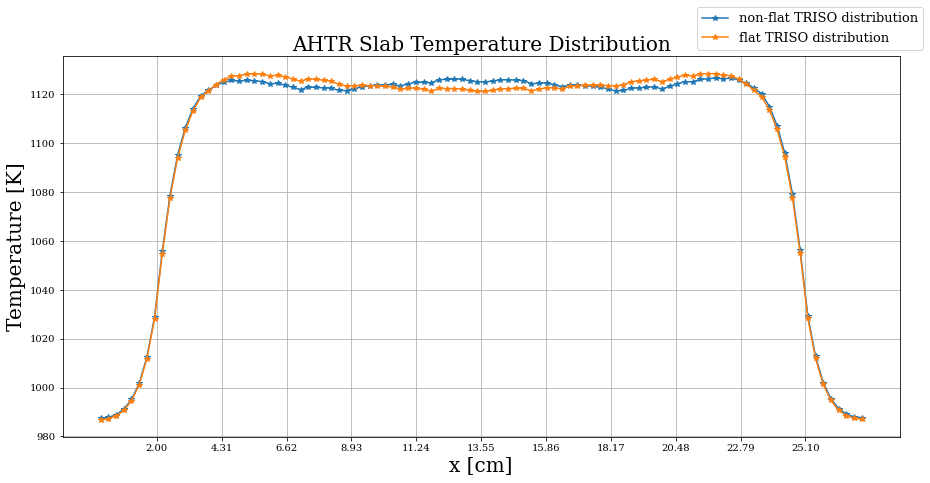
\includegraphics[width=\linewidth]{slab-obj-1-temp-distr.png}
    \caption{Comparison of Moltres-generated AHTR plank temperature distribution for 
    non-flat and flat TRISO distribution. 
    Both models have $PF_{total}$ = 0.0979.}
    \label{fig:slab-obj-1-temp-distr}
\end{figure}
The \gls{AHTR} plank with a flat \gls{TRISO} distribution has higher plank temperatures 
on the left and right sides near the moderator. 
To combat this temperature peak, ROLLO found a \gls{TRISO} distribution that 
has a slight dip near the moderator regions, resulting in a lower $T_{max}$.

\paragraph{Simulation p-1e}
In Section \ref{sec:plank-1-obj-temp}, I conducted single-objective optimization 
simulations to minimize maximum plank temperature ($T_{max}$) while varying coolant 
channel shape. 
In simulation p-1e, \gls{ROLLO} found that there is a negative linear correlation 
between the plank's $T_{max}$ and total radius. 
Comparison of simulation p-1b and p-1e's results in 
Figures \ref{fig:slab-obj-1-temp-evol} and \ref{fig:slab-obj-1-temp-evol-coolant} 
show that coolant channel shape variation does not have as high of an impact on 
$T_{max}$ as \gls{TRISO} distribution variation: the average $T_{max}$ due to 
\gls{TRISO} variation decreased by 60K over 10 generations, while average $T_{max}$ due 
to coolant channel shape variation only decreased by 15K over 10 generations. 

\paragraph{Summary}

\subsection{Discussion: Minimize $PPF_{fuel}$ Objective}
\label{sec:plank-discussion-ppf}
In an effort to understand the motivating factors for the minimize $PPF_{fuel}$ 
objective, I conduct an equation analysis in Section
\ref{sec:plank-discussion-ppf-equation} to determine the \gls{AHTR} plank properties 
that influence $PPF_{fuel}$. 
I also demonstrate the relationship derived for simulation p-1c and p-2b's results. 

\subsubsection{Equation Analysis}
\label{sec:plank-discussion-ppf-equation}
Equation \ref{eq:reaction-rate-fission} shows the relationship between fission reaction 
rate, flux, and material properties. 
\begin{align}
\label{eq:reaction-rate-fission}
    RR_f &= \Phi \times \sigma_f \times N \\
\intertext{where}
    RR_f &= \mbox{fission reaction rate } [reactions \cdot cm^{-3} \cdot s^{-1}] \nonumber \\
    \Phi &= \mbox{neutron flux } [neutrons \cdot cm^{-2} \cdot s^{-1}] \nonumber \\
    \sigma_f &= \mbox{microscopic cross section } [cm^2] \nonumber \\
    N &= \mbox{atomic number density } [atoms \cdot cm^{-3}] \nonumber 
\end{align}

Since microscopic cross section is constant for the same fuel material, we can rearrange 
Equation \ref{eq:reaction-rate-fission} into Equation \ref{eq:reaction-rate-fission-prop}: 
\begin{align}
    \label{eq:reaction-rate-fission-prop}
    \Phi \propto \frac{RR_f}{N}
\end{align}
In Section \ref{sec:ahtr_slab_output}, I defined $PPF_{fuel}$ as: 
\begin{align}
    PPF_{fuel} &= max(\frac{fqr_j}{PF_j}) \div ave(\frac{fqr_j}{PF_j})
\intertext{where}
j &= \mbox{discretized fuel area j} \nonumber \\
PPF_{fuel} &= \mbox{fuel-normalized power peaking factor} \nonumber \\
fqr_j &= \mbox{fission-q-recoverable at position j} \nonumber \\
PF_j &= \mbox{fuel packing fraction at position j} \nonumber
\end{align}
The fission reaction rate ($RR_f$) is proportional to fission energy production rate 
($fqr$). 
The atomic number density (N) is proportional to the fuel packing fraction ($PF$). 
Thus, we can further rearrange Equation \ref{eq:reaction-rate-fission-prop} into 
Equation \ref{eq:flux-prop-fqr}:
\begin{align}
    \label{eq:flux-prop-fqr}
    \Phi_j \propto \frac{fqr_j}{PF_j}
\end{align}
We can further rearrange into Equation \ref{eq:flux-prop-ppf}:
\begin{align}
    \label{eq:flux-prop-ppf}
    max(\Phi_j) \div ave(\Phi_j) &\propto max(\frac{fqr_j}{PF_j}) \div ave(\frac{fqr_j}{PF_j}) \nonumber \\
    &\propto PPF_{fuel}
\end{align}

Therefore, from Equation \ref{eq:flux-prop-ppf}, a flatter flux (smaller 
$max(\Phi_j) \div ave(\Phi_j)$ value) will result in a smaller $PPF_{fuel}$. 
Specifically, flatter Group 4 thermal flux results in a smaller $PPF_{fuel}$
(see Table \ref{tab:fission-flux}). 
Table \ref{tab:fission-flux} shows the percentage contributions of fission reactions from 
each energy group. 
\begin{table}[htbp!]
    \centering
    \onehalfspacing
    \caption{Percentage of fission reactions from each energy group for \gls{AHTR} plank model.}
	\label{tab:fission-flux}
    \footnotesize
    \begin{tabular}{llp{4cm}}
    \hline 
    \textbf{Energy Group} & \textbf{Energy Bounds [MeV]} & \textbf{Percentage of Total Fission Reactions [\%]} \\
    \hline
    1 & $9.1188\times 10^{-3} < E < 2.0000\times 10^1$ & 0.85 \\ 
    2 & $2.9023\times 10^{-5} < E < 9.1188\times 10^{-3}$ & 4.85 \\
    3 & $1.8554\times 10^{-6} < E < 2.9023\times 10^{-5}$ & 4.14 \\
    4 & $1.0000\times 10^{-12} < E < 1.8554\times 10^{-6}$ & 90.14 \\
    \hline
    \end{tabular}
\end{table}
Most fission reactions are occurring in Energy Group 4. 

In the following section, I demonstrate this relationship in simulation p-1c and p-2b's 
results. 

\subsubsection{Results Analysis}
\label{sec:plank-discussion-ppf-results}

\paragraph{Simulation p-1c}
In Section \ref{sec:plank-1-obj-ppf}, I conducted single-objective optimization 
simulations to minimize fuel-normalized power peaking factor ($PPF_{fuel}$). 
In simulation p-1c, \gls{ROLLO} found that for $PF_{total}$ = 0.0979, an \gls{AHTR} 
plank model with TRISO distribution that peaks near the edges of the fuel region of 
the plank and a minimum point in center of the plank with a variation of $\sim0.07$, 
most-minimized $PPF_{fuel}$. 

I ran a simulation for constant $PF_{total}$ = 0.0979 and compared its 
flux to simulation p-1c's most-minimized $PPF_{fuel}$ TRISO distribution to understand 
why the latter enabled a lower $PPF_{fuel}$. 
Figure \ref{fig:triso-0.0979} shows the TRISO distributions for the two compared 
simulations: Figure \ref{fig:slab-obj-1-ppf}'s most-minimized $PPF_{fuel}$
TRISO distribution and the constant $PF_{total}$ = 0.0979 TRISO distribution with 
their $PPF_{fuel}$ values. 
\begin{figure}[htbp!]
    \centering
    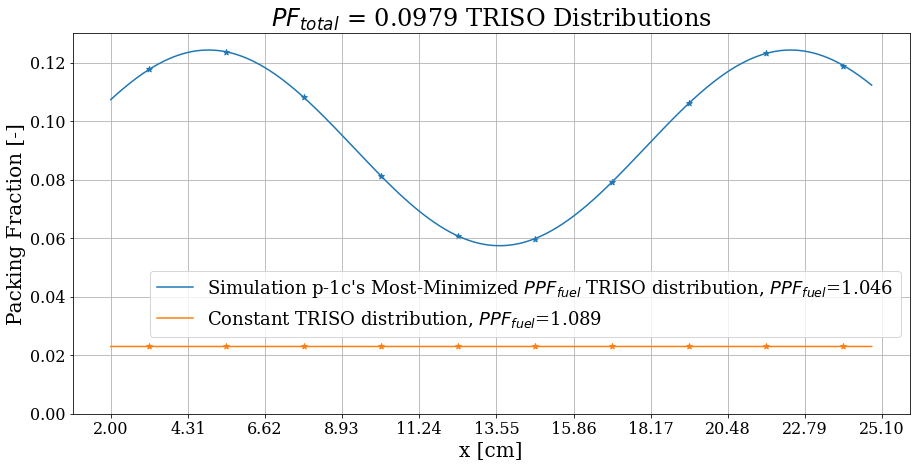
\includegraphics[width=0.9\linewidth]{triso-0.0979.png} 
    \caption{Simulation p-1c's most-minimized $PPF_{fuel}$ TRISO distribution 
    from Figure \ref{fig:slab-obj-1-ppf} and the constant $PF_{total}$ = 0.0979 
    TRISO distribution.}
    \label{fig:triso-0.0979}
\end{figure}

Figure \ref{fig:flux-comparison-0.0979-plank} compares the flux distributions between 
the most-minimized $PPF_{fuel}$ TRISO distribution and a constant $PF_{total}$ = 0.0979 
TRISO distribution (both shown in Figure \ref{fig:triso-0.0979}).
\begin{figure}[htbp!]
    \centering
    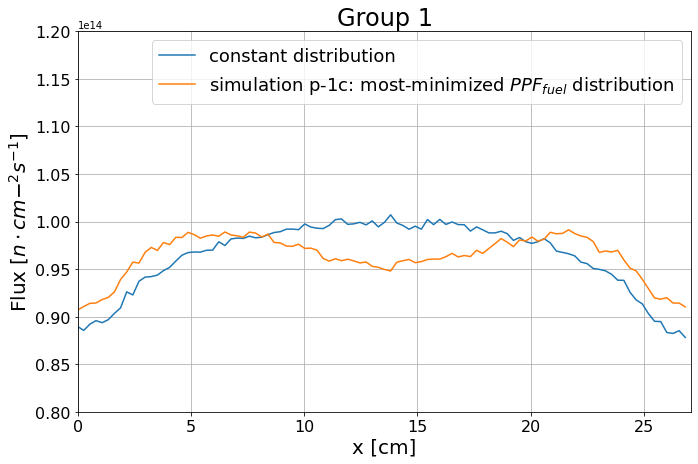
\includegraphics[width=0.48\linewidth]{flux-comparison-0.0979-plank_grp1.png} 
    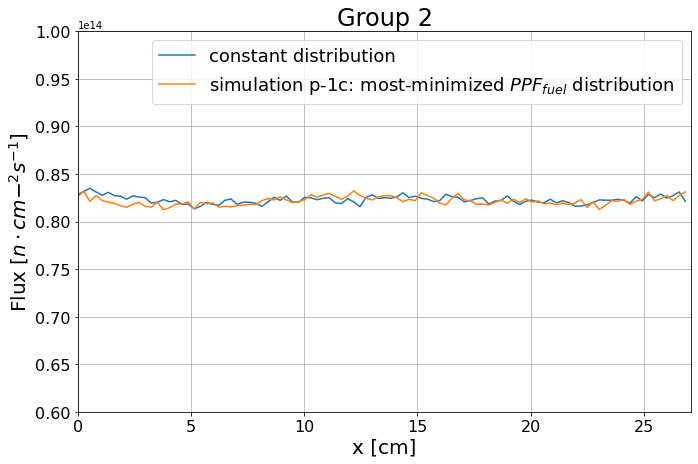
\includegraphics[width=0.48\linewidth]{flux-comparison-0.0979-plank_grp2.png} 
    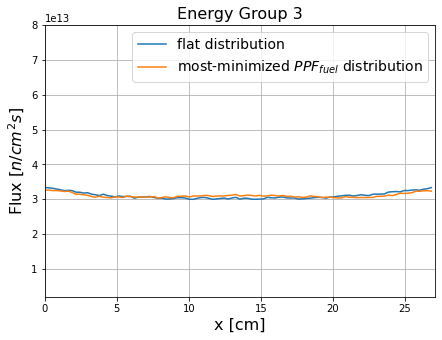
\includegraphics[width=0.48\linewidth]{flux-comparison-0.0979-plank_grp3.png} 
    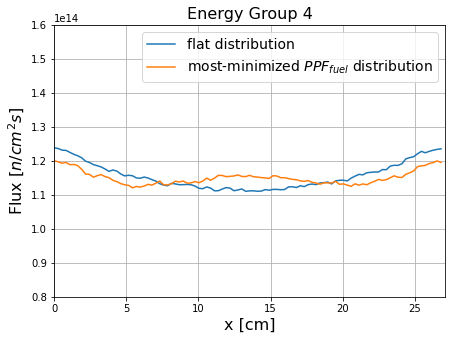
\includegraphics[width=0.48\linewidth]{flux-comparison-0.0979-plank_grp4.png} 
    \caption{Flux comparison between Figure \ref{fig:slab-obj-1-ppf-final}'s TRISO 
    distribution that most-minimized $PPF_{fuel}$ and a constant $PF_{total}$ = 0.0979 
    TRISO distribution. 
    \acrfull{AHTR} plank's centerline neutron flux distribution in 4 groups at 948K. 
    Centerline is the white line in Figure \ref{fig:ahtr-plank-verification}.
    Energy Group 1: E $> 9.1188 \times 10^{-3}$ MeV, 
    Energy Group 2: $2.9023 \times 10^{-5} < E < 9.1188 \times 10^{-3}$ MeV,
    Energy Group 3:  $1.8556 \times 10^{-5} < E < 2.9023 \times 10^{-5}$ MeV,
    Energy Group 4:  $1.0 \times 10^{-12} < E < 1.8554 \times 10^{-6}$ MeV.}
    \label{fig:flux-comparison-0.0979-plank}
\end{figure}
In Figure \ref{fig:flux-comparison-0.0979-plank}, the constant distribution's Group 4 
flux dips in the center of the plank due to spatial self-shielding effects. 
In the Group 1 flux distribution, there is a peak in fast neutrons born in the plank's 
center, they are moderated in the graphite matrix and graphite structure 
(Figure \ref{fig:straightened_plank}). 
The self-shielding neutrons are more likely absorbed at the plank's sides, near 
the pure graphite structure moderating regions. 
The outer sides of the plank geometrically shield the plank's center from neutron 
flux, leading to a relatively lower thermal flux in the plank's center. 

Table \ref{tab:flux-comparison-0.0979-plank} shows quantified flux comparison 
between simulation p-1b's most-minimized $PPF_{fuel}$ TRISO distribution and a constant 
$PF_{total}$ = 0.0979 TRISO distribution (both shown in Figure \ref{fig:triso-0.0979}).
\begin{table}[htbp!]
    \centering
    \onehalfspacing
    \caption{Flux value comparison between Figure \ref{fig:slab-obj-1-ppf-final}'s TRISO 
    distribution that most-minimized $PPF_{fuel}$ and a constant $PF_{total}$ = 0.0979 
    TRISO distribution. 
    Energy Group 1: E $> 9.1188 \times 10^{-3}$ MeV, 
    Energy Group 2: $2.9023 \times 10^{-5} < E < 9.1188 \times 10^{-3}$ MeV,
    Energy Group 3:  $1.8556 \times 10^{-5} < E < 2.9023 \times 10^{-5}$ MeV,
    Energy Group 4:  $1.0 \times 10^{-12} < E < 1.8554 \times 10^{-6}$ MeV.}
	\label{tab:flux-comparison-0.0979-plank}
    \footnotesize
    \begin{tabular}{lp{4cm}p{3.3cm}p{4cm}}
    \hline
    \textbf{Energy Group} &
    \textbf{$max(\phi)/min(\phi)$ most-minimized $PPF_{fuel}$ TRISO distribution} & 
    \textbf{$max(\phi)/min(\phi)$ constant TRISO distribution} & 
    \textbf{$\%$ difference (most minimized - constant)}\\
    \hline 
    1 & 1.093 & 1.147 & \Minus4.68 \\
    2 & 1.024 & 1.027 & \Minus0.22\\
    3 & 1.077 & 1.114 & \Minus3.32 \\
    4 & 1.071 & 1.115 & \Minus3.96 \\
    \hline
    \end{tabular}
\end{table}

In Energy group 4, the most-minimized $PPF_{fuel}$ flux distribution is $3.96\%$ flatter 
than the constant $PF_{total}$ = 0.0979 flux distribution, resulting in a lower 
$PPF_{fuel}$. 

\paragraph{Simulation p-2b}
In Section \ref{sec:p-2b}, I conducted simulation p-2b which is a two-objective 
optimization simulation to minimize fuel-normalized power peaking factor ($PPF_{fuel}$) 
and total fuel packing fraction ($PF_{total}$). 
In simulation p-2b, the TRISO distribution with the most-minimized $PPF_{fuel}$ 
has $PF_{total}$ = 0.0029 and a TRISO distribution that peaks in the center of the plank
and both sides, with a variation of $\sim0.02$.
This distribution differs from simulation p-1c's most-minimized $PPF_{fuel}$ TRISO 
distribution (Figure \ref{fig:slab-obj-1-ppf-final}) which has a large $\sim 0.07$ 
variation in TRISO distribution. 

I ran a simulation for constant $PF_{total}$ = 0.029 and compared its 
flux to simulation p-2b's most-minimized $PPF_{fuel}$ TRISO distribution to understand 
why the latter enabled a lower $PPF_{fuel}$. 
Figure \ref{fig:triso-0.0292} shows the TRISO distributions for the two compared 
simulations: Figure \ref{fig:slab-obj-2-pfppf}'s most-minimized $PPF_{fuel}$
TRISO distribution and the constant $PF_{total}$ = 0.029 TRISO distribution with 
their $PPF_{fuel}$ values. 
\begin{figure}[htbp!]
    \centering
    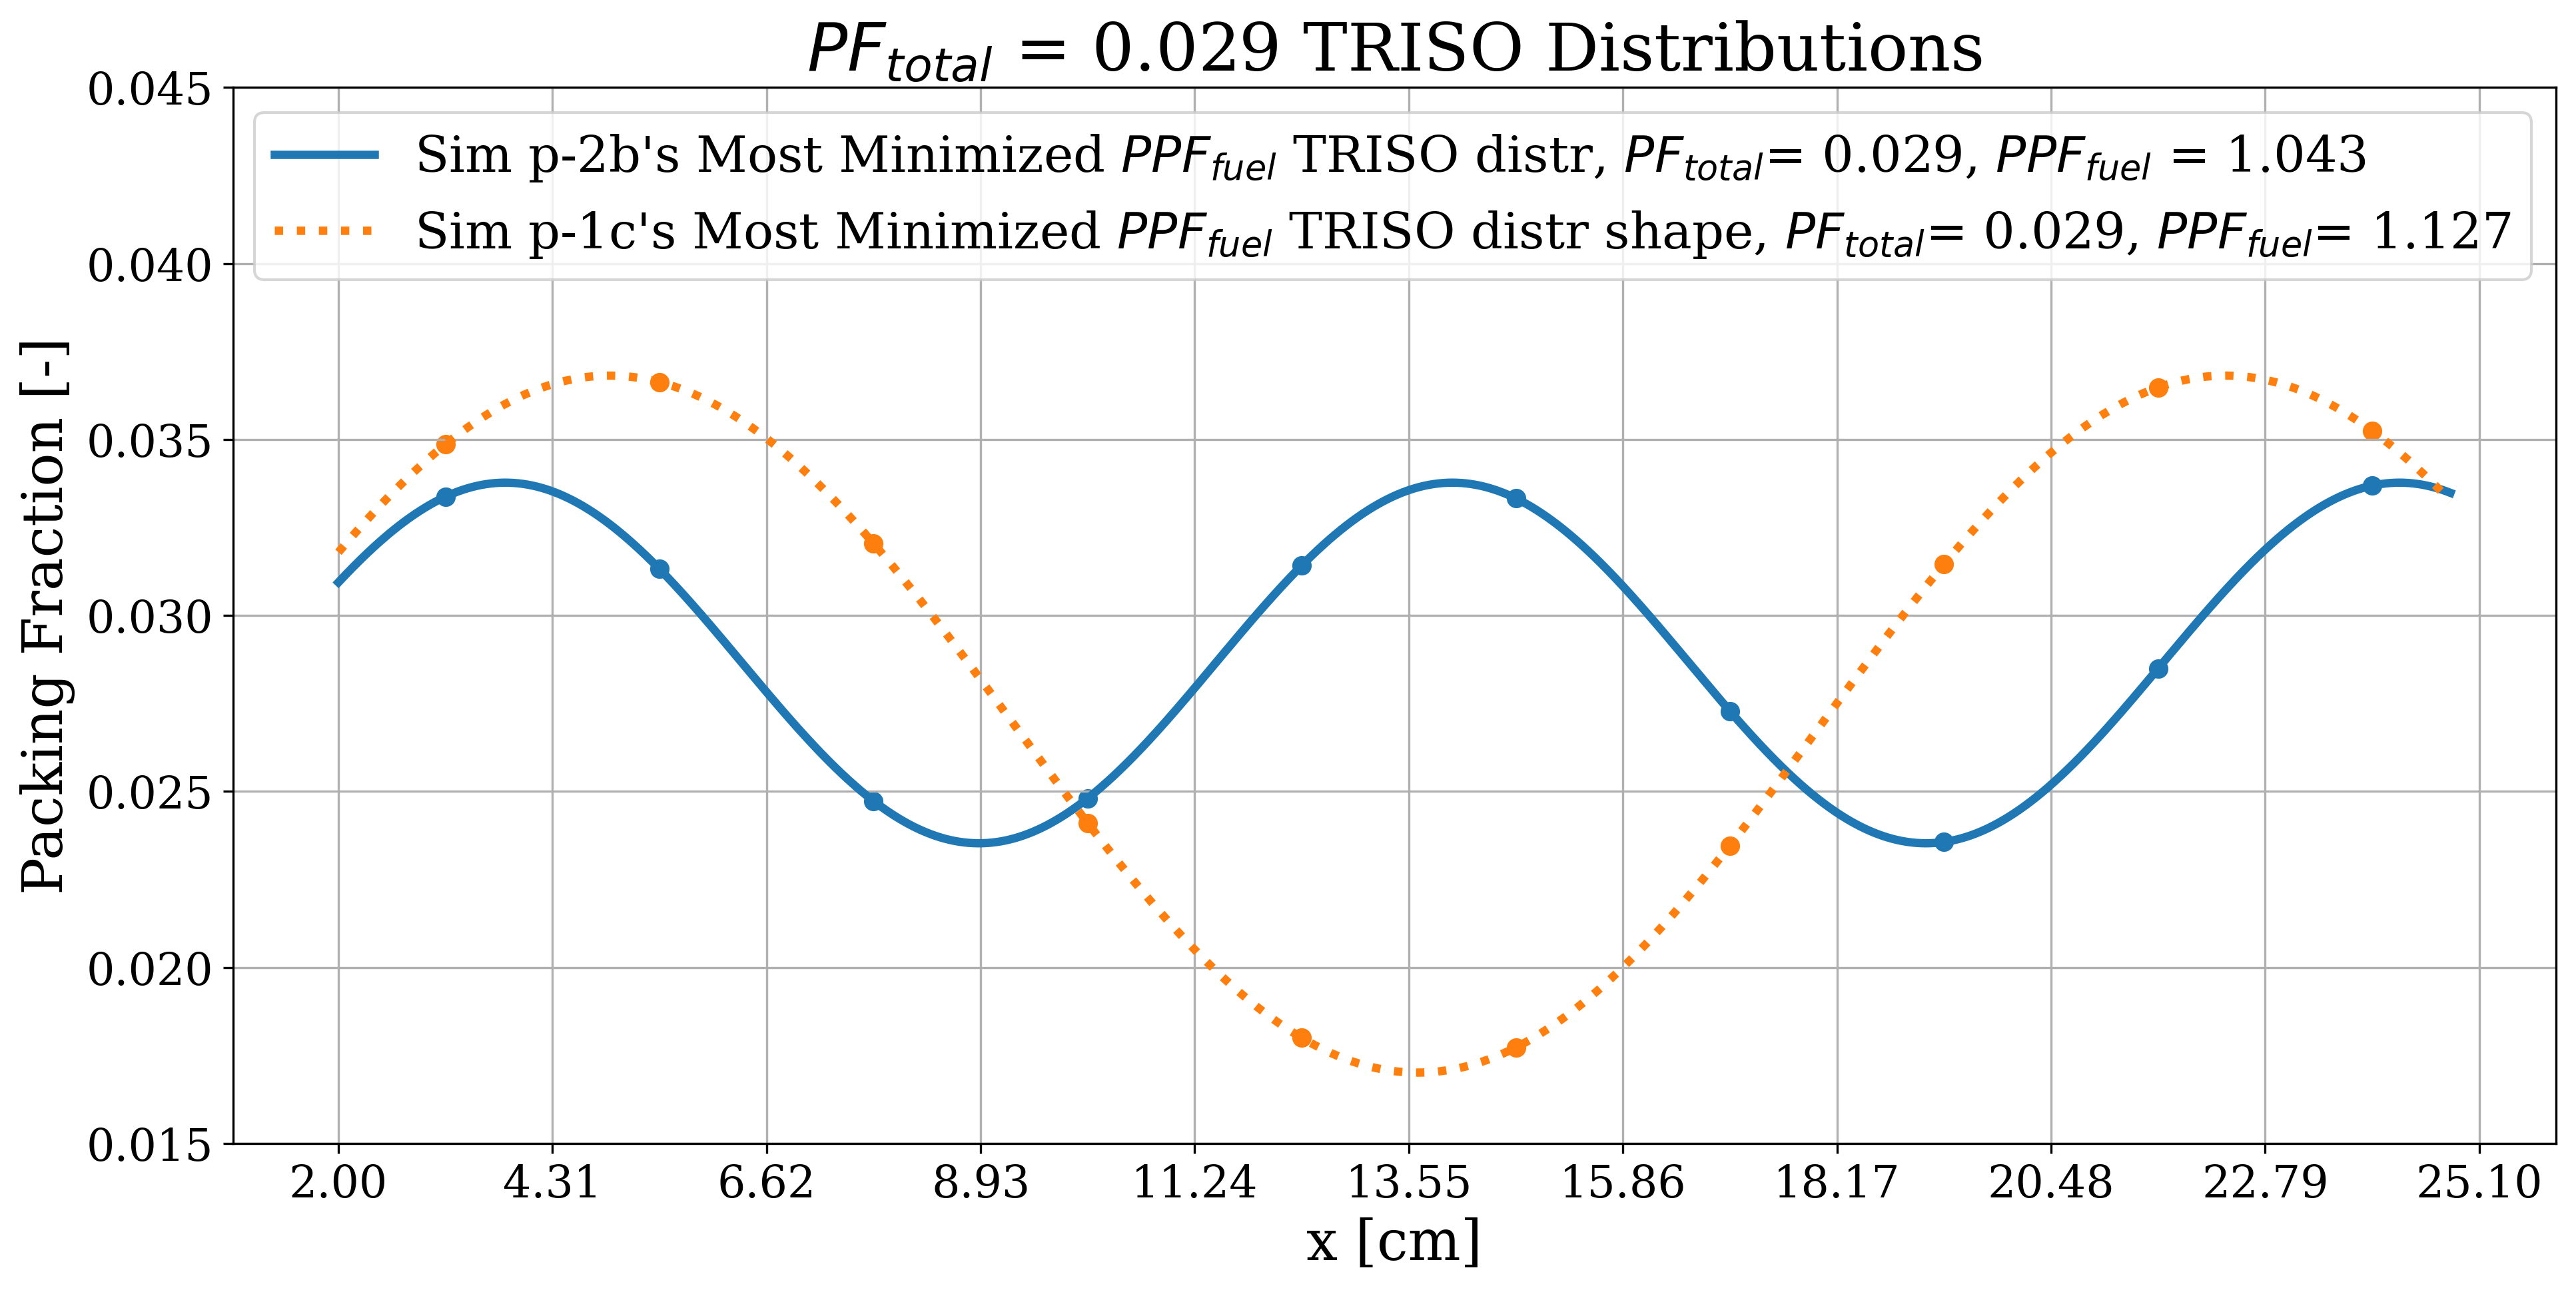
\includegraphics[width=0.9\linewidth]{triso-0.029.png} 
    \caption{Simulation p-2b's most-minimized $PPF_{fuel}$ TRISO distribution 
    from Figure \ref{fig:slab-obj-2-pfppf} and the constant $PF_{total}$ = 0.0292
    TRISO distribution.}
    \label{fig:triso-0.0292}
\end{figure}

Figure \ref{fig:flux-comparison-0.0292-plank} compares the flux distributions between 
simulation p-2b's most-minimized $PPF_{fuel}$ TRISO distribution and a 
constant $PF_{total}$ = 0.0292 TRISO distribution (both shown in Figure 
\ref{fig:triso-0.0292}).
\begin{figure}[htbp!]
    \centering
    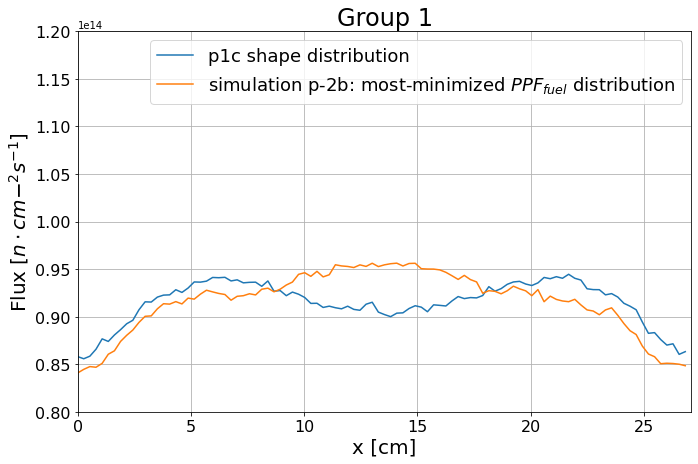
\includegraphics[width=0.48\linewidth]{flux-comparison-0.0292-plank_grp1.png} 
    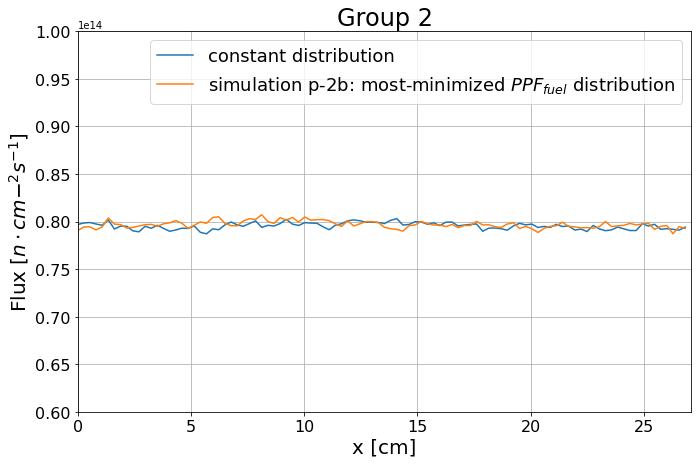
\includegraphics[width=0.48\linewidth]{flux-comparison-0.0292-plank_grp2.png} 
    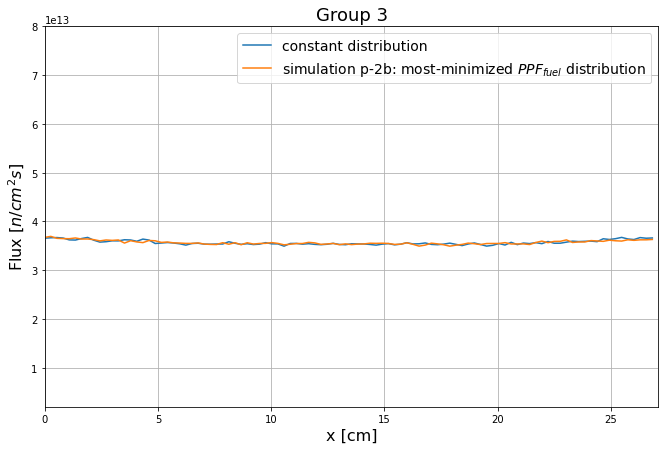
\includegraphics[width=0.48\linewidth]{flux-comparison-0.0292-plank_grp3.png} 
    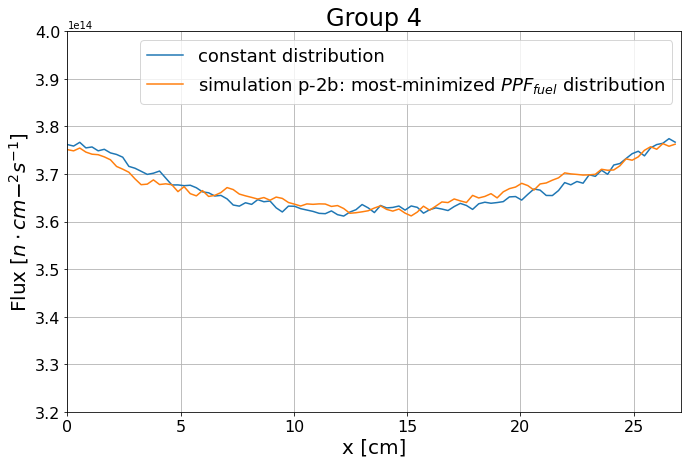
\includegraphics[width=0.48\linewidth]{flux-comparison-0.0292-plank_grp4.png} 
    \caption{Flux comparison between Figure \ref{fig:slab-obj-2-pfppf}'s TRISO 
    distribution that most-minimized $PPF_{fuel}$ and a constant $PF_{total}$ = 0.0292 
    TRISO distribution. 
    \acrfull{AHTR} plank's centerline neutron flux distribution in 4 groups at 948K. 
    Centerline is the white line in Figure \ref{fig:ahtr-plank-verification}.
    Energy Group 1: E $> 9.1188 \times 10^{-3}$ MeV, 
    Energy Group 2: $2.9023 \times 10^{-5} < E < 9.1188 \times 10^{-3}$ MeV,
    Energy Group 3:  $1.8556 \times 10^{-5} < E < 2.9023 \times 10^{-5}$ MeV,
    Energy Group 4:  $1.0 \times 10^{-12} < E < 1.8554 \times 10^{-6}$ MeV.}
    \label{fig:flux-comparison-0.0292-plank}
\end{figure}

Table \ref{tab:flux-comparison-0.0292-plank} shows quantified flux comparison 
between simulation p-2b's most-minimized $PPF_{fuel}$ TRISO distribution and a constant 
$PF_{total}$ = 0.0292 TRISO distribution (both shown in Figure \ref{fig:triso-0.0292}).
\begin{table}[htbp!]
    \centering
    \onehalfspacing
    \caption{Flux value comparison between Figure \ref{fig:slab-obj-2-pfppf}'s TRISO 
    distribution that most-minimized $PPF_{fuel}$ and a constant $PF_{total}$ = 0.0292 
    TRISO distribution. 
    Energy Group 1: E $> 9.1188 \times 10^{-3}$ MeV, 
    Energy Group 2: $2.9023 \times 10^{-5} < E < 9.1188 \times 10^{-3}$ MeV,
    Energy Group 3:  $1.8556 \times 10^{-5} < E < 2.9023 \times 10^{-5}$ MeV,
    Energy Group 4:  $1.0 \times 10^{-12} < E < 1.8554 \times 10^{-6}$ MeV.}
	\label{tab:flux-comparison-0.0292-plank}
    \footnotesize
    \begin{tabular}{lp{4cm}p{3.3cm}p{4cm}}
    \hline
    \textbf{Energy Group} &
    \textbf{$max(\phi)/min(\phi)$ most-minimized $PPF_{fuel}$ TRISO distribution} & 
    \textbf{$max(\phi)/min(\phi)$ constant TRISO distribution} & 
    \textbf{$\%$ difference (most minimized - constant)}\\
    \hline 
    1 & 1.137 & 1.152 & \Minus1.31 \\
    2 & 1.025 & 1.020 & \Plus0.49 \\
    3 & 1.057 & 1.051 & \Plus0.56 \\
    4 & 1.042 & 1.045 & \Minus0.28 \\
    \hline
    \end{tabular}
\end{table}

In Energy group 4, the most-minimized $PPF_{fuel}$ flux distribution is $0.28\%$ flatter 
than the constant $PF_{total}$ = 0.0292 flux distribution, resulting in a lower 
$PPF_{fuel}$. 
In the previous section, simulation p-1c's most-minimized $PPF_{fuel}$ flux 
distribution is $3.96\%$ flatter than the constant $PF_{total}$ = 0.0979 flux 
distribution with $\sim 0.07$ variation in TRISO distribution. 
This contrasts with simulation p-2b's $\sim 0.02$ variation in TRISO distribution. 
Higher $PF_{total}$ in simulation p-1b means that there is more fuel, resulting in 
higher self-shielding effects. 
This results in TRISO distribution variation having a stronger effect in neutralizing 
self-shielding. 

\paragraph{Simulation p-1f}
In Section \ref{sec:plank-1-obj-ppf}, I conducted single-objective optimization 
simulations to minimize fuel-normalized power peaking factor ($PPF_{fuel}$) while 
varying coolant channel shape. 
Comparison of simulation p-1c and p-1f's results in Figures 
\ref{fig:slab-obj-1-ppf-evol-coolant} and \ref{fig:slab-obj-1-ppf-evol}
show that coolant channel shape variation barely has an impact on $PPF_{fuel}$ as 
\gls{TRISO} distribution variation: the average $PPF_{fuel}$ due to \gls{TRISO} 
variation decreased by 0.1 over 10 generations, while average $PPF_{fuel}$ due to 
coolant channel shape variation only decreased negligibly over 10 generations. 
Figure \ref{fig:slab-obj-1-ppf-final-coolant} reiterates that there is no correlation 
between total radius and $PPF_{fuel}$. 

\paragraph{Summary}
Therefore, I conclude that the minimize $PPF_{fuel}$ objective is driven by flattening 
thermal (Group 4) flux. 

\subsection{Discussion: Multi-Objective Optimization}
\gls{ROLLO} successfully finds widely spread solutions in each of the multi-objective 
optimization final generation's Pareto front.
\gls{ROLLO} is a global search of a large design space and helps narrow down possible 
solutions.
This informs reactor designers of optimal reactor parameters for their defined objectives.  
From here, reactor designers can conduct sensitivity analysis and use high fidelity 
models to characterize a smaller section of the design space.

\section{Summary}